\chapter{Universal Module}\label{chap:universal_module}

Chapter \ref{chap:rofi} gives the specification for modules in the RoFI
platform. In this chapter, we present the RoFI \emph{universal module}. This
module is supposed to be the primary building block of RoFI systems. It should
provide enough versatility to build a broader range of systems.

This chapter provides an overview of the design of the universal module and
gives a specification to implement it. The current state of implementation is
discussed in chapter \ref{chap:prototypes}.

\section{Universal Module Shape}

The universal RoFI module occupies two adjacent cells of the grid as can be seen
in figure \ref{fig:um_reference}. Please note that this drawing gives a
simplified model in which many technical details are omitted. The arrangement of
the module is inspired by the M-TRAN \cite{kurokawa_distributed_2008}. Unlike
M-TRAN, the universal module is grid-aware. The module composes of four parts:
\begin{enumerate*}
    \item \emph{body A},
    \item \emph{body B},
    \item \emph{shoe A}, and
    \item \emph{shoe B}.
\end{enumerate*}
See figure \ref{fig:um_body_parts}. Bodies are supposed to encapsulate
actuators, electronics, and accumulators; shoes are meant to provide connection
to other modules and provide movement.

\begin{figure}[t]
    \centering
    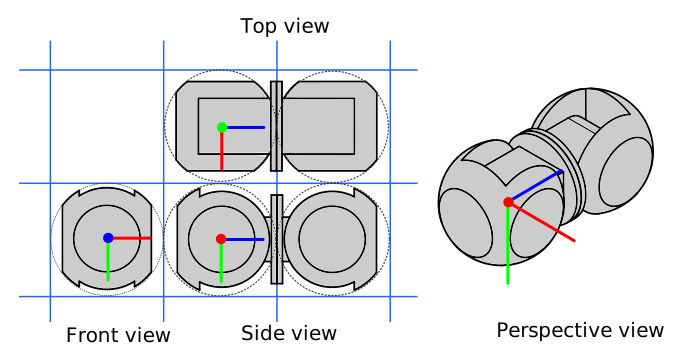
\includegraphics[width=\textwidth]{figures/um_reference.pdf}
    \caption{The universal RoFI module. Blue lines specify the grid, dotted
    lines marks spheres in which the module in inscribed. Note that we show the
    module with the Z axe facing right as it better fits  the page layout. }
    \label{fig:um_reference}
\end{figure}

\begin{figure}[t]
    \centering
    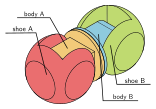
\includegraphics[width=0.7\textwidth]{figures/um_body_parts.pdf}
    \caption{Parts of the universal module.}
    \label{fig:um_body_parts}
\end{figure}

There are 3 degrees of freedom (figure \ref{fig:um_axis}):
\begin{enumerate}
    \item shoe A can rotate against body A along the $\alpha$ axe in a range
    $\langle -90^\circ; +90^\circ\rangle$,
    \item shoe B can rotate against body B along the $\beta$ axe in a range
    $\langle -90^\circ; +90^\circ\rangle$, and
    \item body A can rotate against body B along the $\gamma$ axe in $\langle
    -180^\circ; +180^\circ\rangle$ with an overflow\footnote{First prototypes
    feature a limitation on a number of overflows in one direction on the
    $\gamma$ axe due to technical limitations. }.
\end{enumerate}
The module should be able to provide at least 1.5 $\text{N}\cdot\text{m}$ of
torque for each axe.

\begin{figure}
    \centering
    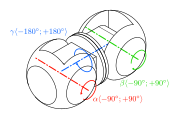
\includegraphics[width=0.7\textwidth]{figures/um_axis.pdf}
    \caption{Degrees of freedom of the universal module. The figure represents
    neutral position of each joint.}
    \label{fig:um_axis}
\end{figure}

There are 3 docks on each shoe -- docks $X+, X-$ and $Z-$. The position of the
docks is captured in figure \ref{fig:um_docks}. The shape descriptor in figure
\ref{fig:um_descriptor} captures the universal module arrangement.

\begin{figure}
    \centering
    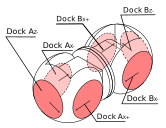
\includegraphics[width=0.7\textwidth]{figures/um_docks.pdf}
    \caption{Docks on the universal module. The arrow on each dock specifies its orientation.}
    \label{fig:um_docks}
\end{figure}

Such a module arrangement is more versatile than to the M-TRA arrangement.
Addition of the third axe, the $\gamma$ axe, overcomes two limitations of
M-TRAN-like arrangement:
\begin{enumerate*}
    \item given a chain configuration with all joints parallel to each other,
    the system can span only in two dimensions; it cannot expand into the third
    dimension.
    \item Also, given a ring configuration which can roll forward, the M-TRAN
    module cannot steer and only moves forward.
\end{enumerate*}


\section{Universal Module Sensors}

We design the universal module to be rather sensor-impecunious rather than
sensor-rich. There should be various RoFI systems with various sensor needs.
Therefore, we find much useful to implement in the universal module only sensors
that can be beneficial nearly in all systems. The special sensors for concrete
systems should be implemented as separate modules.

There are two types of sensors in each universal module:
\begin{enumerate*}
    \item inertial measurement unit (IMU) and
    \item distance sensors in the middle of each dock.
\end{enumerate*}
The IMU provides a basic notion of the module orientation in the space. Data
from IMU can be used in algorithms to, e.g., determine a common direction in
space among all modules using the Earth's gravitational force. A good solution
for the IMU IC is MPU-9250 \cite{noauthor_mpu-9250_2016} due to broad community
support and all-in-one-package solution (accelerometer, gyroscope, and
magnetometer).

We plan to use the VL53L1X \cite{noauthor_new_2018} time-of-flight distance
sensor in each dock. The sensors allow the universal module to detect obstacles
in front of the module, help to establish correct alignment of two docks when
connecting and can also be used to scan the environment. The scanning of the
environment is performed by moving a shoe and building a depth map. The depth
map can be used as a simple input for computer vision. For example, when the
RoFI system is supposed to climb the stairs, it can measure their geometry by
this procedure.

\section{Intra-module Architecture}

Each universal module is an autonomous unit. A single \emph{control unit}
controls the module. This unit controls all the other components of the module
as can be seen in figure \ref{fig:um_internal}. The unit controls smart
servomotors over a bus built on top UART, docks over SPI bus and directly
controls charging and power management circuits.

\begin{figure}
    \centering
    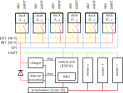
\includegraphics[]{figures/um_internal.pdf}
    \caption{Block diagram of internal architecture of the module.}
    \label{fig:um_internal}
\end{figure}

\subsection{Control Unit}

The control unit is designed to be powered by the ESP32 microcontroller
\cite{noauthor_esp32_2018}. This microcontroller provides enough computational
power, provides rich peripherals including Bluetooth 4 Low Energy and WiFi
802.11 b/g/n, and most importantly, the vendor provides excellent software
support. We are mainly concerned by three aspects of the software support:
\begin{enumerate*}
    \item there is support for modern C/C++ compilers with full support for the
    C++ standard library (including exception handling and concurrency),
    \item the development framework provides POSIX compatible interface, and
    \item there is a vendor maintained port of the lwIP library.
\end{enumerate*}

First two aspects are crucial for easy development of software. From a practical
aspect, the ESP32 is nearly indistinguishable from a desktop POSIX environment
while it still preserves real-time nature and easy access to low-level
peripherals. The POSIX compatibility allow the developers to leverage existing
libraries and port them to the universal module without a significant effort.
The support for lwIP is a benefit as the control unit serves as network
switch (as defined in section \ref{sec:communication}) and therefore, we can
use it. The only necessary part of implementing is the custom device driver for the
docks.

The control unit is not supposed to provide any sensors except the IMU since the
placement of IMU in the robot is not crucial. The distance sensors on the docks
are controlled by a microcontroller on the dock and the control unit.


\subsection{Motors}

We decided to use so-called \emph{smart servomotors} (servos) to power the
universal module. These servos are similar to their hobby counterparts. Just
like the hobby servo, a smart servo is a DC motor with a gearbox combined with a
driver and feedback loop controller in a single compact package. The main
difference between these two is that smart servos provide a digital bus for
sending commands (unlike pulse-width modulation communication used in hobby
servos) and offer several advanced features. The hobby servo can be controlled
only in position mode without any feedback to the control system. The smart
servos usually allow for multiple control modes (torque, speed, and position),
allow continuous rotation and also provide feedback to the control system.
Therefore, the system can detect when the motor reaches a commanded
position or if the motor is overloaded.

The usage of smart servos simplifies both, the mechanical construction and the
control unit, as we can omit motor driver, custom gearing and encoders. In our
design, we use HerkuleX DRS-0101 \cite{noauthor_herkulex_nodate} servos. These
servos are designed to be powered directly from a two cell li-ion accumulator
and provide 1.2 N$\cdot$m of torque at maximal speed one turn per second. The
servos communicate over UART bus, where the control unit serves as a master and
the servos are slaves. The servos can be daisy-chained and therefore, only two
wires are required for the communication. The command set provides means to
perform a synchronized movement.

We choose the DRS-0101 servos for several reasons: they feature slightly smaller
mechanical size compared to the Dynamixel AX-12A \cite{noauthor_dynamixel_2006}
(a comparable servo), they are mechanically compatible with DRS-0201
\cite{noauthor_herkulex_nodate} servos, which feature twice the power. The servo
is also mechanically compatible with Lewansoul LX-16A
\cite{noauthor_lx-16a_2018}, which is a low-cost alternative for possible future
mass production.

\subsection{Power Management}

The module is supposed to be powered from a two cell li-ion accumulator pack.
The motors can directly operate from the accumulator at their rated voltage and
can drain sufficient current. The control unit is also powered from the
accumulator.

The internal connection of power rails is captured in figure
\ref{fig:um_internal}. There is a charger circuit to allow for charging from the
INT line. The charger is controlled by the control unit -- it can be either
disabled or it can charge the accumulator with given power limit. There is also
a step-up convertor used to source power to other modules. The used step-up
convertors must be parallelizable (denoted by a diode in the block diagram). The
step-up module is also controlled by the control unit and can be disabled when
not needed.

Provided this power sharing setup, the module can operate in four modes:

\paragraph{Self-powered mode} The module runs on its own accumulator (charger is
disabled and convertor is disabled).

\paragraph{Power sourcing mode} The module provides energy to the network
(charger is disabled and convertor is enabled).

\paragraph{Power draining mode} The module charges its accumulator and drains
power from other modules.

\paragraph{Survivor mode} The module disables motors, disables converter and
limits the charging power roughly to cover energy consumption of the control
module. Therefore, no charging occurs and the charger is acts as a step-down
converter for the control unit.

The communication in the RoFI platform requires an activity from the control
unit as it routes packets between the docks. If a module shuts down due to
discharged accumulator, there cannot be any communication across the module.
Dead module might lead to a separation of the system into two independent
networks in some configurations. Charging the dead module might not be strategic
in many cases. Therefore, survivor mode can be applied to keep the communication
going without waisting power on charging the dead module.

\section{RoFI Program Interface}

We expect the firmware to be developed using standard programming means for the
ESP32 microcontroller. That is the firmware is developed using C++ facilitated
by the ESP-IDF \cite{noauthor_esp-idf_nodate} framework. The framework provides
drivers for MCU peripherals, FreeRTOS, the standard C and C++ libraries, and
also offers several useful libraries (lwIP for network communication, Bluetooth
library or library for virtual file system). The framework exposes its
functionality as a plain C interface. In addition, many of the provided
functionality is also wrapped in POSIX-compatible interface. E.g, sockets are
accessible by both, lwIP interface and POSIX interface. The same follows for
threading; user can use FreeRTOS API or can leverage POSIX interface or can even
use C++ STL API.

The ESP32 provides sufficient tools for software development using stand modern
means. However, this means only cover general software development needs. We do
not want the user to write a custom library for controlling the motors, docks
and other. Therefore, the universal module should also provide \emph{RoFI
Driver}, a software library which provides interface to RoFI specific tasks.

The RoFi Driver consists of three parts: \todo{XXX}.

\subsection{The RoFI "BIOS"}

\subsection{Reactive Blocks Library}

Software development for robots and embedded systems is considered to be more
challenging than a classical software development. There are several reasons
why the development is challenging:
\begin{enumerate*}
    \item the microcontroller peripherals have to be mastered,
    \item testing and debugging is harder as the system is not self-contained a
    interacts with the environment, and
    \item the code has to deal with numerous asynchronous events and there task
    which needs to be distributed in time.
\end{enumerate*}

The challenge of mastering complicated peripherals can be mitigated by writing a
suitable high level drivers. Such drivers provide abstraction and hide
implementation on the hardware level. Therefore the user does not need to toggle
individual bits in configuration registers. Also the peripherals of modern
microcontrollers are more powerful and general and therefore, allow for good
abstraction. ESP-IDF provides such drivers for ESP32.

The burden of testing robotic software can be partially mitigated by splitting
the software into two layers -- the control layer operating on top an
input/output layer. The I/O layer interacts with peripherals drivers, interacts
with the environment and provide rather high level inputs to the control layer.
With setup it is possible to mock-up the I/O layer and perform standard software
testing of the control layer. However, testing is still rather challenging and
we do not bring any innovation in this field.

There are currently two classical approaches to tackle the burden of handling
asynchronous events in languages like C or C++. First, a real-time operating
system (RTOS) can be used with several tasks. Each task handles events in
synchronous, blocking, manner. This approach leads to a readable code as the
logic for handling events is kept close together and follows chronological flow
of the events. However, it might not preserve the lowest possible latency due to
RTOS task switching and also does not scale well as each the number of tasks is
usually limited. The second approach uses callback functions which are called to
handle an event. This approach scales well, however it leads to hard-to read
code as the callbacks do not preserve context and are spread all over the source
code. This phenomenon is usually referred as ``callback hell''. Also, code
complexity increases tremendously when error handling is added.

We designed a new solution for handling asynchronous events for the RoFI
platform. We call it \emph{reactive blocks}. The idea behind reactive blocks is
simple -- we use the same principle as callbacks, however, we provide a
syntactical sugar to write them in a chain-like structure to preserve the
chronological flow of event handling. Reactive blocks are inspired by the
ReactiveX library \cite{noauthor_reactivex_nodate} and the ranges-v3 library
\cite{noauthor_range-v3_nodate}.

The reactive blocks will be implemented as a stand-alone RoFi independent C++
library -- \emph{Ractive Blocks Library} (RBL). The library targets all
platforms with C++17 support and STL support. This includes standard variants of
x64, ARM and also embedded platform like ESP32 a or ARM COrtex-M. As the library
implementation is a subject of another thesis, we provide only a brief
description of its core functionality and omit the implementation details.

Consider following (rather artificial) scenario: when a noisy distance sensor
overcomes a given threshold (generates edge), the robot notifies several other
robots (judges) over a network. The judges vote and if a majority votes yes, the
robot flashes a LED. For simplicity, consider a line-based text communication
protocol between the robots and numerous reasonably named functions.

Standard implementation using blocking interface might look like this:
\begin{minted}{cpp}
while ( true ) {
    // Wait rising edge debounced by 10 samples
    ring_buffer< int > samples( 10, 0 );
    while ( !all( samples,
                  []( int x ){ return x > threshold; } ) )
    {
        samples.push( sensor.read() );
        delay( 10_ms );
    }
    int sensorValue = average( samples );

    // Perform voting
    std::vector< bool > votes;
    for ( auto& judge : judges ) {
        judge.send( "value: " + std::to_string( sensorValue ) )
        vote = judge.receiveLine() == "yes";
        votes.push_back( vote );
    }

    // Flash an LED
    if ( majority( votes, []( bool vote ){ return vote; } ) ) {
        led.on();
        delay( 200_ms );
        led.off();
    }
}
\end{minted}

The sample code is straightforward and easily readable. By putting the code in a
separate task, we can handle multiple asynchronous events simultaneously.
However, the code does is not efficient as possible as the network communication
is synchronous.

Each asynchronous function traditionally takes a callback function as its
argument. The callback is called, when the operation is finished. The result
value or error is passed to the callback. The task from our example scenario
could be implemented like this using asynchronous interface:

\begin{minted}{cpp}
std::vector< bool > votes;
template < typename Callback >
void onJudgeResponse( const std::string& resp, Callback c ) {
    votes.push_back( resp == "yes" );
    if ( votes.size() == judges.size() &&
         majority( votes, []( bool vote ){ return vote; } ) )
    {
        c();
    }
}

template < typename Callback >
void vote( int value, Callback c ) {
    for ( auto& judge : judges ) {
        judge.send( "value: " + std::to_string( sensorValue ), [=] {
            judge.receiveLine( [=]( const std::string& s ) {
                onJudgeResponse( resp, s, c );
            } );
        } );
    }
}

ring_buffer< int > samples( 10, 0 );
timer.every( 10_ms. [&ring_buffer]() {
    samples.push( sensor.read() );
    if ( all( samples,
        []( int x ){ return x > threshold; } ) )
    {
        vote( average( samples ), judges, []{
            led.on();
            timer.after( 200_ms, []{
                led.off();
            });
        });
    }
});
\end{minted}

The code is now fully asynchronous, but is hard to read -- it does not preserve
the chronological order of event handling, the user have to think about shared
states and has a lot of nested sections. The need for a shared state arises from
the absence of information in the control flow of the program. E.g, the function
\texttt{onJudgeResponse} has to check if it is the last call of the function. In
the first example there is no such need as the the control captures the
information -- once the if-clause is reached, it is clear all judges voted.

The solution we provide is shown in code snippet below. We do not expect the
reader to immediately understand all the details of the code:

\begin{minted}{cpp}
auto overThreshold( std::pair< int, int > value ) {
    return value.first > threshold;
}

auto is( const std::string& what ) {
    return [=]( const std::string& s ) { return s == what; }
}

auto setLed( bool value ) {
    return [=]() { led.set( value ) };
}

auto sensorStream = timer.every( 20_ms ) >> sensor.read;
auto sensorAverage = sensorStream >> slidingAverage( 10 );
zip( sensorStream, sensorAverage)
    >> debounceOn( overThreshold )
    >> std::get< 1 >
    >> [&]( int value ) {
        return for_each( judges, [=]( auto& judge ) {
            std::string msg =
                "value: " + std::to_string( sensorValue );
            return judge.send( message )
                    >> judge.receiveLine >> is( "yes" );
        } ) >> majority;
    }
    >> setLed( true ) >> wait( 200_ms ) >> setLed( false );
\end{minted}

The reactive blocks follow similar idea as the range-v3 library -- we describe a
pipeline for data transformation, however unlike ranges-v3, the data might be
scattered over time. By describing the pipeline the user can preserve
chronological ordering of the event handling in the code but also preserves
asynchronicity at the same time.

Reactive blocks allow to chain data transformation operations. Each operation is
represented by a block. There are two type of blocks:
\mintinline[breaklines]{cpp}{template < typename T > Puslisher< T > } and
\mintinline[breaklines]{cpp}{template < typename T > Subscriber< T > }. Single
block can be both publisher and subscriber.

\noindent The publisher can:
\begin{enumerate}
    \item emit an arbitrary number of values of type \texttt{T} at any time,
    \item emit an error (object inheriting from
    \mintinline[breaklines]{cpp}{std::exception}), and
    \item close itself. After closing no more values nor errors can be emitted.
\end{enumerate}

\noindent The subscriber can subscribe to a to publisher. After subscribing it
\begin{enumerate}
    \item receives values of type \texttt{T} emitted by the publisher and
    \item can unsubscribe.
\end{enumerate}

These operations are sufficient to implement chaining of the blocks. Consider
following, low level code snipper:
\begin{minted}{cpp}

\end{minted}


\subsection{RoFI Driver}

\subsection{Remote Procedure Call}